\subsection{Разработка интерфейса взаимодействия}

Графический интерфейс пользователя, согласно выбору архитектуры клиент-сервер, основывается на технологии HTML + CSS + JavaScript с использованием Ajax запросов. 

\subsubsection{Разработка графа диалога}

Разработаем верхний уровень графа диалога с пользователем:
\begin{itemize}
\item \textbf{Главный экран} -- должен содержать элементы интерфейса для наиболее часто используемых функций АИС. Так как основной функцией АИС является поиск по новостным документам, то главный экран содержит рубрикатор, форму ввода поискового запроса и результат выполнения поискового запроса.
\item \textbf{Экран импорта} -- должен содержать элементы интерфейса для добавления документов в систему, а именно: форму ручного ввода, импорт архива документов и управление автоматизированным импортом документов из папки импорта.
\item \textbf{Экран экспорта} -- должен содержать элементы интерфейса для экспорта документов из системы.
\item \textbf{Экран управления} -- должен содержать элементы интерфейса для управления длительными операциями над индексом документов, над рубрикатором и другими действиями с предоставлением информации о прогрессе операции.
\item \textbf{Экран настроек} -- должен содержать элементы интерфейса для изменения и просмотра пользовательских настроек системы.
\item \textbf{Экран прогноза} -- должен содержать элементы интерфейса для отображения графиков активности новостных потоков, графики прогноза их активности, оценку качества прогноза и результирующую аналитическую функцию прогноза.
\end{itemize}

Обобщенный граф диалога представлен на рисунке~\ref{figure:dialog_generic}.

\clearpage
\begin{figure}[h!]
\centering
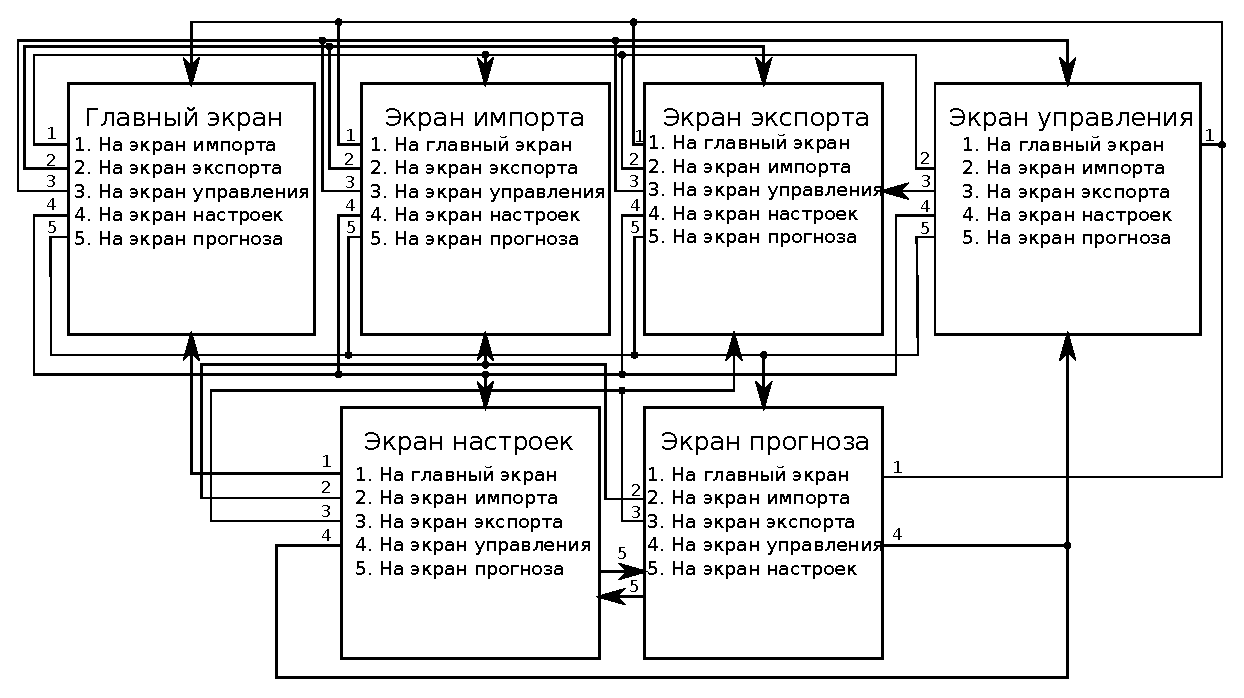
\includegraphics[angle=90,origin=c]{technology/dialog_generic}
\caption{Обобщенный граф диалога взаимодействия с пользователем}
\label{figure:dialog_generic}
\end{figure}

\clearpage
\subsubsection{Разработка экранных форм}

При разработке экранных форму учитывались следующие требования к интерфейсу:
\begin{itemize}
\item Интерфейс должен быть удобен как для квалифицированного персонала, так и для новых пользователей АИС.
\item На каждом основном экране АИС должно присутствовать меню для перехода на другие экраны системы.
\item На каждом экране должны присутствовать только те элементы интерфейса, что необходимы для решения задачи, для которой экран предназначен.
\item Ввод данных должен быть интерактивным, то есть проводить проверку корректности вводимой информации и отображать причину ошибки в случае неправильно сформированных данных.
\end{itemize}

Основные экранные формы представлены в графической части проекта.

\clearpage
\subsection{Описание экранных форм}

\subsubsection{Главный экран}

\begin{figure}[h!]
\centering
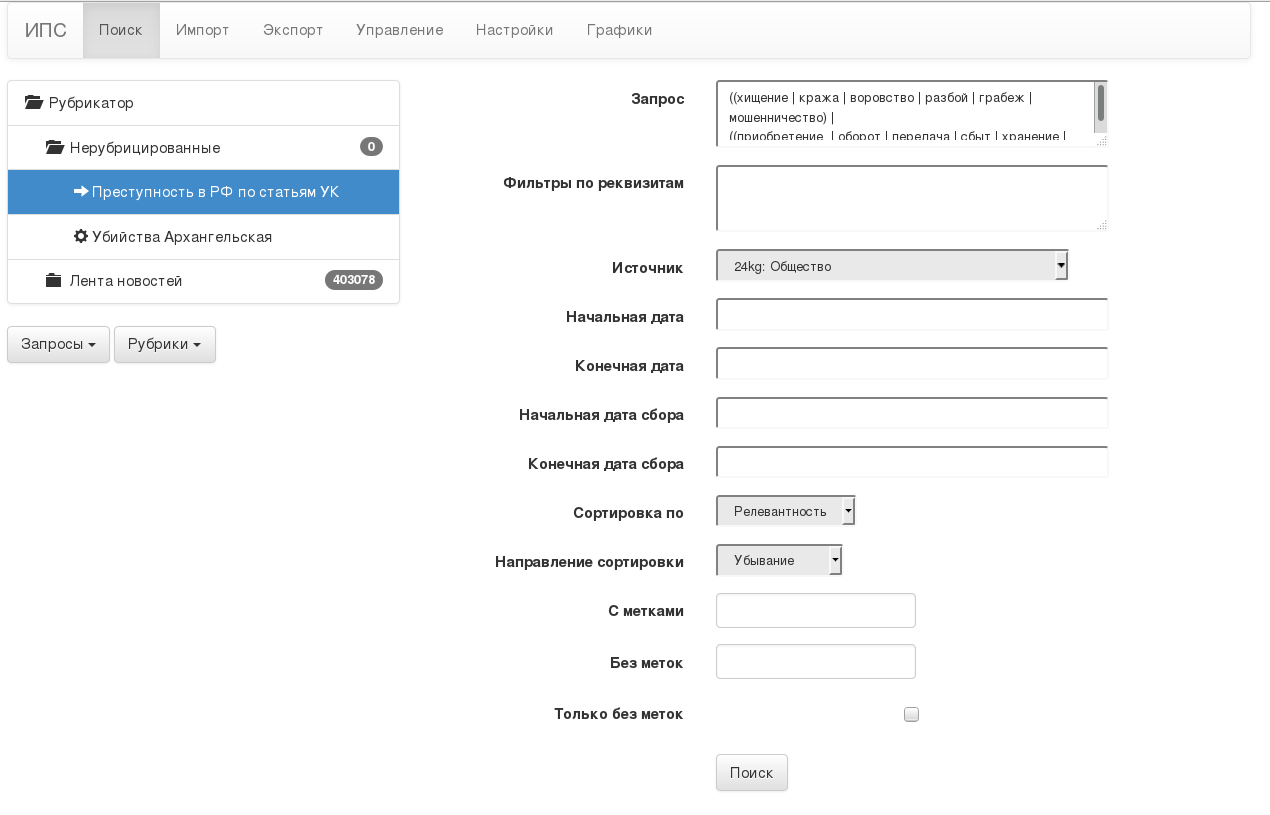
\includegraphics[width=0.9\linewidth]{technology/gui_main}
\caption{Главный экран АИС}
\label{figure:guiMain}
\end{figure}

На рис.~\ref{figure:guiMain} представлен вид главного экрана АИС. Экран содержит:
\begin{itemize}
\item Меню в главной части, через которое можно попасть на другие экраны системы.
\item Рубрикатор в левой части экрана. Через рубрикатор пользователь может выбирать текущие категории документов, выбирать сохранённые запросы. Выпадающие панели под рубрикатором содержат действия над рубриками (создание, обновление, удаление, перемещение, экспорт из рубрики) и над сохранёнными запросами (создание, обновление, удаление). Рядом с названиями рубрик отображается количество документов в рубрике.
\item Форма ввода запроса в правой части экрана. В форме присуствуют следующие поля:
\begin{enumerate}
\item Запрос -- тело формализованного запроса;
\item Фильтры по реквизитам -- дополнительные ограничения на реквизиты документа;
\item Источник -- выпадающий список из всех доступных источников документов;
\item Начальная дата -- фильтрация по дате публикации документа. Задает начальное значение интервала;
\item Конечная дата -- фильтрация по дате публикации документа. Задает конечное значение интервала;
\item Начальная дата сбора -- фильтрация по дате сбора документа. Задает начальное значение интервала;
\item Конечная дата сбора -- фильтрация по дате сбора документа. Задает конечное значение интервала;
\item Сортировка по -- указание реквизита документа, по которому будет проводиться сортировка;
\item Направление сортировки -- указание направления сортировки, по убыванию или по возрастанию;
\item С метками -- перечисление меток документа, которые должны у него присутствовать;
\item Без меток -- перечисление меток документа, которые должны у него отсутствовать;
\item Только без меток -- специальный признак, при активации которого поиск будет проводиться только по документам, у которых нет никаких меток;
\end{enumerate}

\end{itemize}

\begin{figure}[h!]
\centering
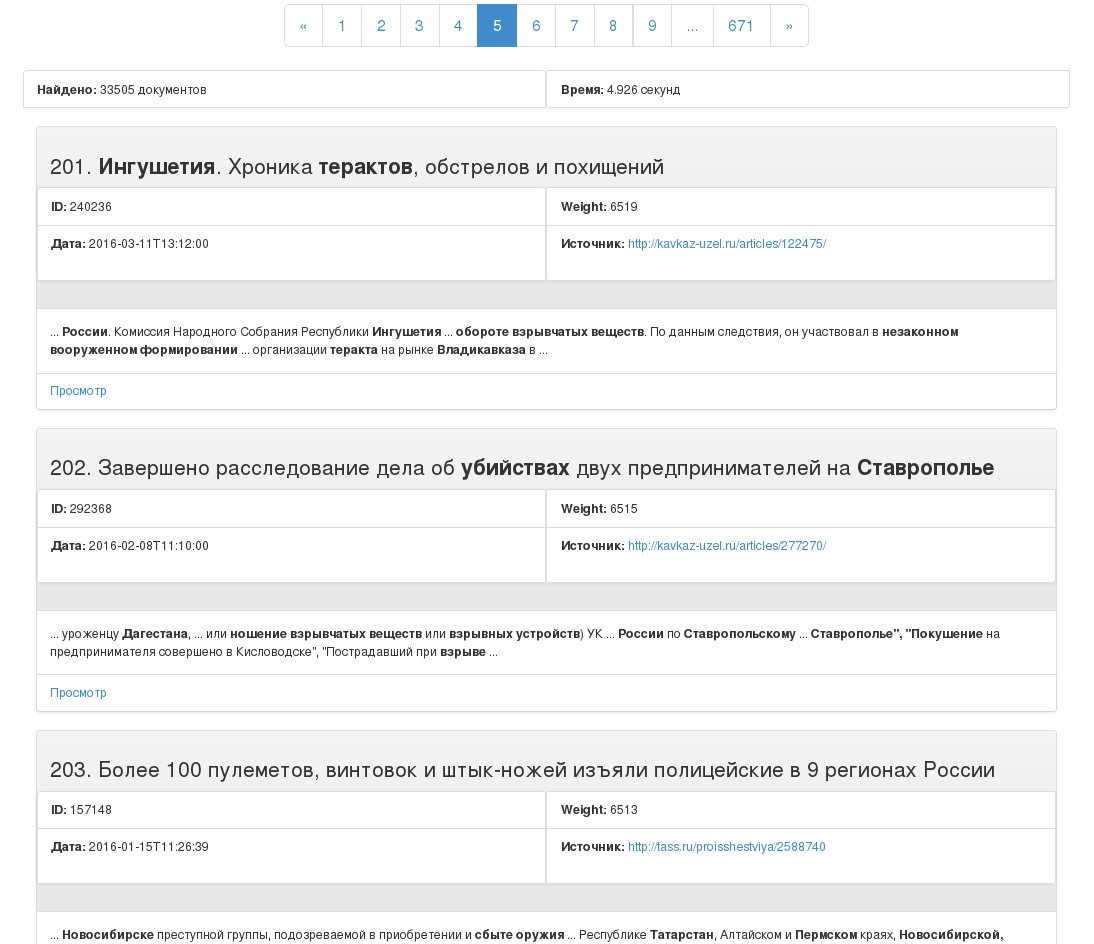
\includegraphics[width=0.9\linewidth]{technology/gui_main_results}
\caption{Главный экран АИС, поисковая выдача}
\label{figure:guiMainResults}
\end{figure}

После нажатия на кнопку <<Поиск>> в нижней части экрана пользователю отображается вторая часть данного экрана с поисковой выдачей (рис.~\ref{figure:guiMainResults}). Поисковая выдача может содержать множество документов, поэтому экран содержит кнопки перехода по страницам. Каждый элемент выдачи содержит название документа, его основные реквизиты и кусок текста, который подходит под заданный формализованный запрос. 

\begin{figure}[h!]
\centering
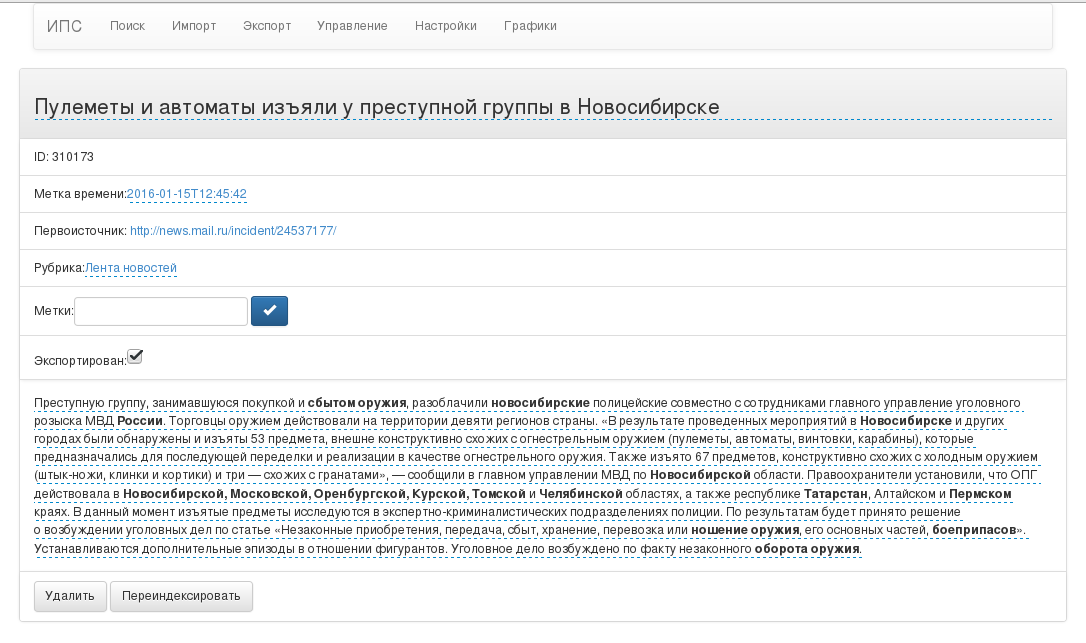
\includegraphics[width=0.9\linewidth]{technology/gui_main_document}
\caption{Просмотр полного документа}
\label{figure:guiMainDocument}
\end{figure}

Документ в элементе поисковой выдачи можно просмотреть отдельно с помощью ссылки <<Просмотр>> в нижней части элемента выдачи. Вид страницы документа представлен на рис.~\ref{figure:guiMainDocument}. Подробный вид документа содержит значения всех реквизитов, а также предоставляет возможность удаления или переиндексирования документа. Каждый реквизит, кроме идентификатора и источника, можно отредактировать путем щелчка мышкой на данных реквизита и ввода новых во всплывающем элементе ввода. Текст документа подсвечен согласно последнему выполненному запросу.

\clearpage
\subsubsection{Экран импорта}

\begin{figure}[h!]
\centering
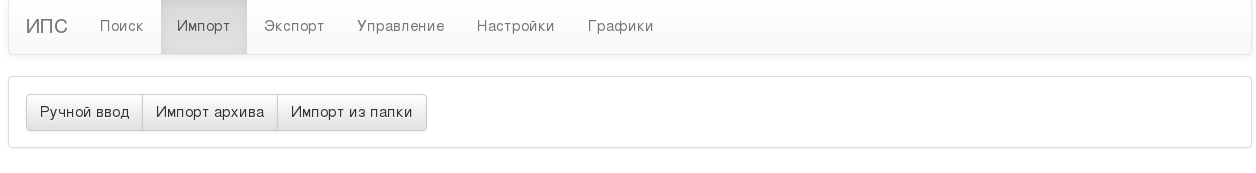
\includegraphics[width=0.9\linewidth]{technology/gui_import}
\caption{Экран импорта документов}
\label{figure:guiImport}
\end{figure}

На рис.~\ref{figure:guiImport} представлен вид экрана импорта документов. Экран содержит:
\begin{itemize}

\end{itemize}

\clearpage
\subsubsection{Экран экспорта}

\begin{figure}[h!]
\centering
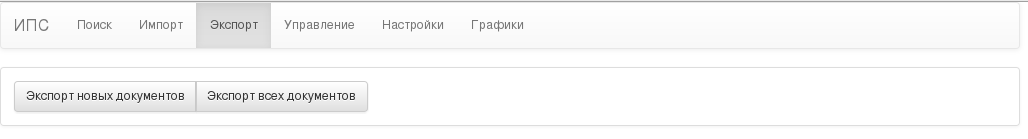
\includegraphics[width=0.9\linewidth]{technology/gui_export}
\caption{Экран экспорта документов}
\label{figure:guiExport}
\end{figure}

На рис.~\ref{figure:guiExport} представлен вид экрана экспорта документов. Экран содержит:
\begin{itemize}

\end{itemize}

\clearpage
\subsubsection{Экран управления}

\begin{figure}[h!]
\centering
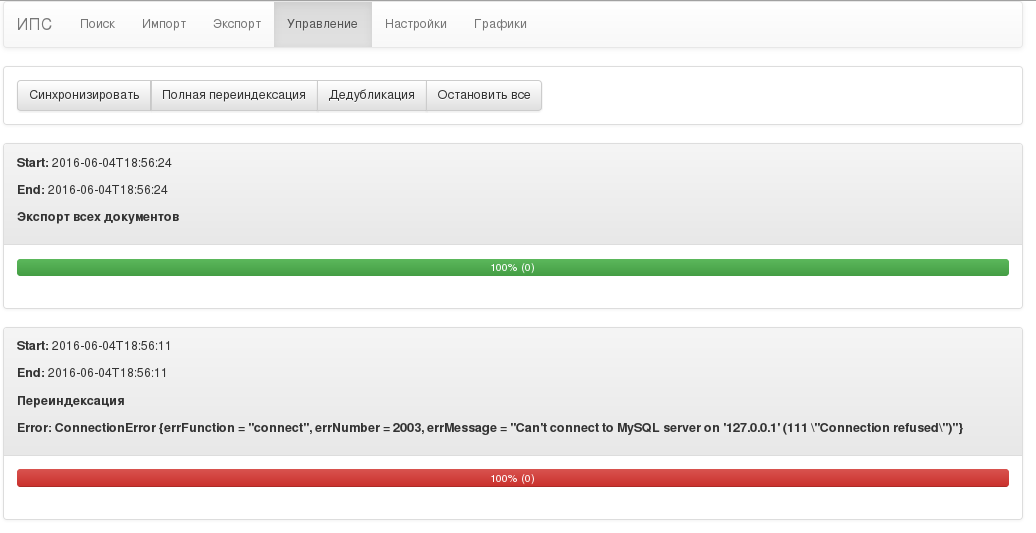
\includegraphics[width=0.9\linewidth]{technology/gui_resync}
\caption{Экран управления операциями АИС}
\label{figure:guiResync}
\end{figure}

На рис.~\ref{figure:guiResync} представлен вид экрана управления операциями АИС. Экран содержит:
\begin{itemize}

\end{itemize}

\clearpage
\subsubsection{Экран настроек}

\begin{figure}[h!]
\centering
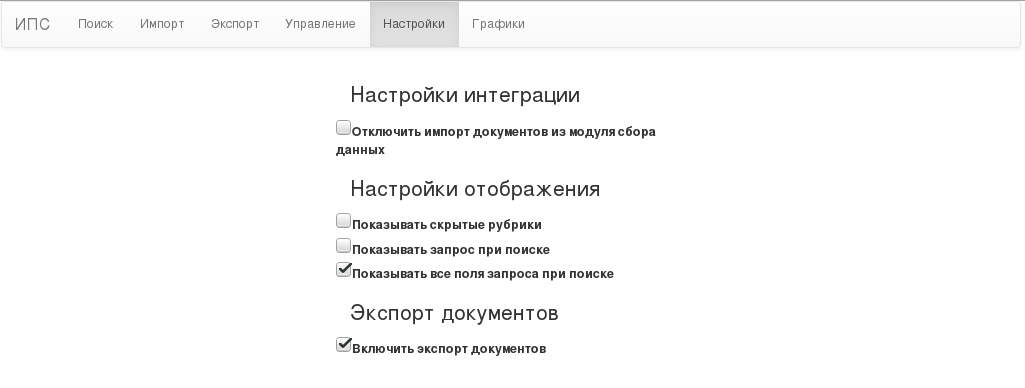
\includegraphics[width=0.9\linewidth]{technology/gui_options}
\caption{Экран настроек АИС}
\label{figure:guiOptions}
\end{figure}

На рис.~\ref{figure:guiOptions} представлен вид экрана настроек АИС. Экран содержит:
\begin{itemize}

\end{itemize}

\clearpage
\subsubsection{Экран прогнозирования} 

\begin{figure}[h!]
\centering
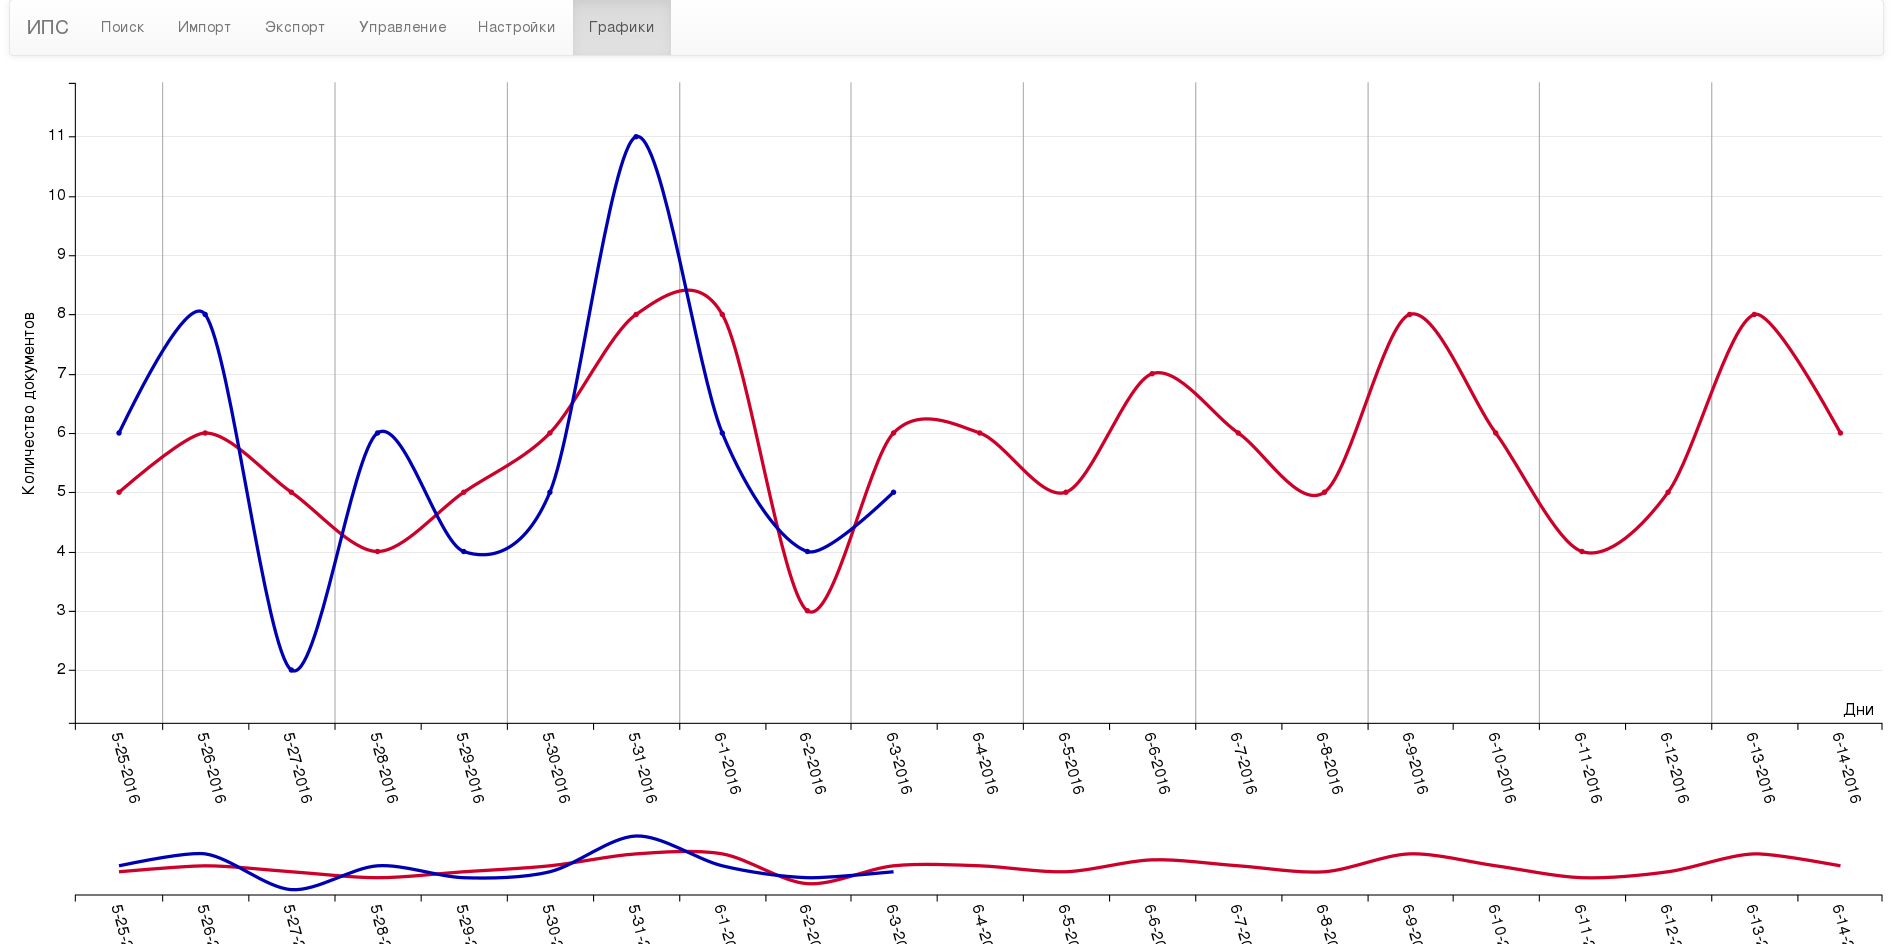
\includegraphics[width=0.9\linewidth]{technology/gui_predict1}
\caption{Экран прогнозирования АИС}
\label{figure:guiPredict}
\end{figure}

На рис.~\ref{figure:guiPredict} представлен вид экрана прогнозирования АИС. Экран содержит:
\begin{itemize}

\end{itemize}
